\section{Modulübersicht}
Die App besteht aus vier Modulen, die sich gemäß MVP einer der Rollen Model, View oder Presenter zuordnen lassen. Dabei unterteilen sich komplexere Module in weitere Unterpakete. Die Presenter-Rolle wird durch das ApplicationLogic Modul~\eqref{module:applicationlogic} realisiert. Das Utils-Modul~\eqref{modules:utils} unterstützt es dabei mit grundlegenden Operationen und Datenstrukturen. Als Model agieren die Module ServerAccess~\eqref{modules:serveraccess} und MemoryAccess~\eqref{modules:memoryaccess}. Schaubild \ref{fig:modules_overview} veranschaulicht die Einteilung:
\begin{figure}[ht]
	\centering
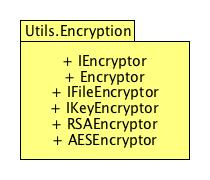
\includegraphics[width=1\textwidth]{./resources/Diagramme/App/modules_overview.jpg}
\caption{Module der Android App}
	\label{fig:modules_overview}
\end{figure}
\newpage
\subsection{ApplicationLogic} \label{module:applicationlogic}
Im Paket ApplicationLogic befinden sich sämtliche Activities und Fragments sowie die CameraView. Diese Komponenten stehen in direkter Verbindung zur Benutzeroberfläche und reagieren auf Nutzereingaben. In diesem Paket befindet sich ebenfalls das Unterpaket ApplicationLogic.Camera, welches Klassen zur Instanzierung und Kontrolle der Kamera beinhaltet. Die Klasse CameraView befindet sich nicht in diesem Unterpaket, da sie eine SurfaceView ist und, wie die Fragments und Activities, direkt vom Nutzer zu sehen ist und die Kamera verwendet, anstatt sie bereitzustellen. ApplicationLogic.Camera beinhaltet nur die Klassen, die auch von anderen Komponenten verwendet werden können, um auf die Kamera zugriff zu erhalten.
\newpage
\subsection{MemoryAccess}  \label{module:memoryaccess}
Das Paket MemoryAccess regelt zugriffe auf den internen Speicher des Android Geräts. Dazu gehört neben dem Speichern von Dateien auch der Zugriff auf die von Android bereitgestellten SharedPreferences. Ebenfalls in dieser Klasse enthalten sind POJOs die aus den vom Speicher gelesenen Daten erstellt werden und anderen Komponenten so ihre Informationen in gebündelter Form verfügbar machen.
\newpage
\subsection{ServerConnection} \label{module:serverconnection}
Das ServerConnection Paket enthält alle Klassen die notwendig sind, um Anfragen an den Web Dienst zu senden und dessen Antwort zu empfangen. dazu gehört der entsprechende Proxy sowie die Klassen zur Herstellung der Verbindung und Weiterreichung der Antwort an die aufrufende Klasse.
\newpage
\subsection{Utils} \label{module:utils}
Das Utils Paket ist in zwei weitere Unterpakete Aufgeteilt: Utils.DataStructures enthält Datenstrukturen wie den Ringbuffer sowie Klassen, die notwendig sind, um Inhalte der Datenstrukturen in den Speicher des Geräts zu übertragen. Hierbei handelt es sich lediglich um die dafür erforderliche Logik. Die Speicherung übernimmt schlißlich das MemoryAccess Modul.